\documentclass[
  11pt,
  letterpaper,
   addpoints,
   answers
  ]{exam}

\usepackage{../exercise-preamble}
\usepackage{multicol}
\begin{document}

\noindent
\begin{minipage}{0.47\textwidth}

\includegraphics[width=\textwidth]{../fcfm_die}
\end{minipage}
\begin{minipage}{0.53\textwidth}
    
\begin{center} 
\large\textbf{Análisis y Diseño de Circuitos Eléctricos} (EL3101-2) \\
\large\textbf{Clase auxiliar 8} \\
\normalsize Prof.~Santiago Bradford V.\\
\normalsize Prof.~Aux.~Erik Saez A. - Rodrigo Catalán\\
             - Byron Castro R.
\end{center}
\end{minipage}

\vspace{0.5cm}
\noindent
\vspace{.85cm}

\begin{questions}

    %%%%%%%%%%%%%%%%%%%%%%%%%%%%
    \question  Encuentre la función de transferencia \( H(s) = \frac{V_{\text{out}}(s)}{V_{\text{in}}(s)} \) para el circuito de la Figura 2. Indique la naturaleza del filtro y su frecuencia de corte (\( \omega_c \)).

  \begin{center}
        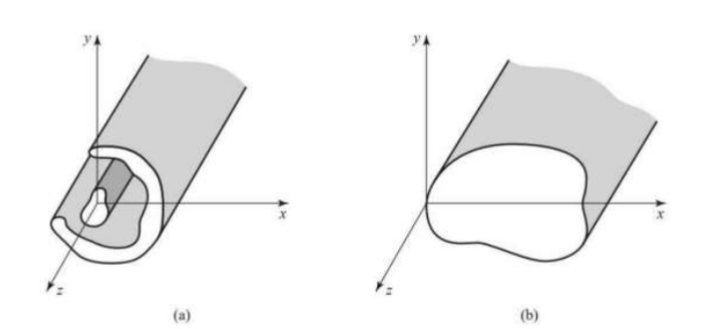
\includegraphics[width=0.45\textwidth]{Auxiliar_8_1}
        \captionof{figure}{Esquema del circuito}
    \end{center}

%%%%%%%%%%%%%%%%%%%%%%%%%%%%%
\begin{solution}
   Las dos inductancias del circuito original están conectadas en serie, por lo que pueden reemplazarse por una única inductancia equivalente cuya inductancia es la suma de ambas. El proceso de reducción se muestra a continuación:

\begin{center}
\begin{circuitikz}
    % Inductancias en serie a la izquierda
    \draw (0,0) to[L, l=20~H] (0,2)
          to[L, l=30~H] (0,4);
    % Nodo con equivalencia
    \node at (1.6,2) {\Large$\Longleftrightarrow$};
    % Inductancia equivalente a la derecha
    \draw (4,0) to[L, l=50~H] (4,4);
\end{circuitikz}
\end{center}

Así, la combinación de una bobina de \( 20\,\mathrm{H} \) en serie con una de \( 30\,\mathrm{H} \) es equivalente a una sola bobina de \( 50\,\mathrm{H} \). Luego, el circuito se simplifica a una resistencia de \( 1\,\text{k}\Omega \) y una inductancia de \( 50\,\mathrm{H} \) en serie. La función de transferencia \( H(s) = \frac{V_{out}}{V_{in}}\) se calcula aplicando la ley de voltajes de Kirchhoff en el dominio de Laplace:

\begin{align}
    -V_{\text{in}}(s) + 10^{3}\,I(s) + 50s\,I(s) &= 0 \\
    (1000 + 50s)I(s) &= V_{\text{in}}(s) \\
    I(s) &= \frac{V_{\text{in}}(s)}{1000 + 50s}
\end{align}
El voltaje de salida $V_{out}$corresponde a la caída de voltaje sobre la inductancia:

\begin{equation}
    V_{\text{out}}(s) = 50s\, \cdot I(s) = 50s \cdot \left(\frac{V_{\text{in}}(s)}{1000 + 50s}\right)
\end{equation}

Por lo tanto, la función de transferencia es:

\begin{align}
    H(s) &= \frac{V_{\text{out}}(s)}{V_{\text{in}}(s)} = \frac{50s}{1000 + 50s} = \frac{s}{s + 20}
\end{align}
Recordando que los filtros pasa altos tienen la forma \( H(s) = \frac{s}{s + \omega_c} \), donde \( \omega_c \) es la frecuencia de corte, podemos identificar que este circuito es un filtro pasa-altos de primer orden con una frecuencia de corte de \( \omega_c = 20\,\mathrm{rad/s} \).

Sea el caso en que las inductancias fueran reemplazadas por condensadores, las dos capacitancias están en serie, por lo que pueden reemplazarse por una única capacitancia equivalente usando la relación:

\[
\frac{1}{C_{\text{eq}}} = \frac{1}{1\,\mu\text{F}} + \frac{1}{3\,\mu\text{F}} = \frac{1 + 3}{3} = \frac{4}{3}
\]
\[
C_{\text{eq}} = \frac{3}{4}\,\mu\text{F} = 0{,}75\,\mu\text{F}
\]

Este proceso de reducción puede representarse así:

\begin{center}
\begin{circuitikz}
    % Condensadores en serie a la izquierda
    \draw (0,0) to[C, l=1~$\mu$F] (0,2)
          to[C, l=3~$\mu$F] (0,4);
    % Nodo con equivalencia
    \node at (1.5,2) {\Large$\Longleftrightarrow$};
    % Condensador equivalente a la derecha
    \draw (4,0) to[C, l=0.75~$\mu$F] (4,4);
\end{circuitikz}
\end{center}
Luego, el circuito se reduce a una resistencia de \( 1\,\text{k}\Omega \) en serie con un condensador de \( 0,75\,\mu\text{F} \).Luego pasamos el condensador al dominio de laplace en el cual su impendancia es \( Z_C(s) = \frac{1}{sC} = \frac{1}{0{,}75\times10^{-6}s} = \frac{4 \cdot 10^{6}}{3s} \),
Planteamos la ecuación de mallas en el dominio de Laplace.
\begin{align}
    -V_{\text{in}}(s) + 10^{3} I(s) + \frac{4 \cdot 10^{6}}{3s} I(s) &= 0
\end{align}
Esto se puede reescribir como:
\begin{align}
   \left[\frac{10^3 \cdot 3s + 4 \cdot 10^{6}}{3s}\right] I(s) = V_{\text{in}}(s)
\end{align}
Con lo que la corriente \( I(s) \) es:
\begin{equation}
    I(s) = \frac{3s}{10^3 \cdot 3s + 4 \cdot 10^{6}} V_{\text{in}}(s)
\end{equation}
Luego considerando que el voltaje $V_{\text{out}}(s)$ es la caída de tensión sobre el condensador, tenemos que:
\begin{equation}
    V_{\text{out}}(s) = \frac{4 \cdot 10^{6}}{3s} I(s) = \frac{4 \cdot 10^{6}}{3s} \cdot \frac{3s}{10^3 \cdot 3s + 4 \cdot 10^{6}} V_{\text{in}}(s)
\end{equation}
Por lo tanto, la función de transferencia es:
\begin{align}
    H(s) &= \frac{V_{\text{out}}(s)}{V_{\text{in}}(s)} = \frac{4 \cdot 10^{6}}{10^3 \cdot 3s + 4 \cdot 10^{6}} = \frac{4 \cdot 10^{6}}{3000s + 4 \cdot 10^{6}}
\end{align}
Dividiendo numerador y denominador por \( 3000 \), tenemos que:
\begin{align}
    H(s) = \frac{ \frac{4 \cdot 10^{6}}{3000}}{\frac{3000s + 4 \cdot 10^{6}}{3000}} = \frac{1333{,}33}{s + 1333{,}33}
\end{align}
La forma de un filtro pasa bajo es \( H(s) = \frac{K}{s + \omega_c} \), donde \( K \) es una constante y \( \omega_c \) es la frecuencia de corte. En este caso, \( K = 1333{,}33 \) y \( \omega_c = 1333{,}33\,\text{rad/s} \). En conclusión, el sistema se comporta como un filtro pasa-bajo RC de primer orden con \( \omega_c \approx 1333\,\text{rad/s} \).

\end{solution}
%%%%%%%%%%%%%%%%%%%%%%%%%%%%%
\question Dada la siguiente función de transferencia:
\begin{equation}
    T(s) = \pm \frac{300(s + 10)}{s(s + 200)}
\end{equation}

Para ello:
\begin{enumerate}
    \item Indique si se trata de un filtro pasa-altos, pasa-bajos, pasa-banda o rechaza-banda.
    \item Diseñe un circuito que permita obtener la función de transferencia \(T(s)\).
\end{enumerate}
%%%%%%%%%%%%%%%%%%%%%%%%%%%%%
\begin{solution}
    \begin{enumerate}
        \item Dada la siguiente función de transferencia:
\begin{equation}
    T(s) = \pm \frac{300(s+10)}{s(s+200)}
\end{equation}

Recordemos que cuando se trabaja con filtros, se estudia el régimen permanente transitorio, por lo que se evalúa la función de transferencia en \( s = j\omega \) dado que solo nos interesa el analisis en frecuencia.
\begin{align}
    T(j\omega) &= \pm \frac{300(j\omega + 10)}{j\omega (j\omega + 200)}
\end{align}

Para analizar el comportamiento en frecuencia, usamos el módulo de la función de transferencia:
\begin{align}
    |T(j\omega)| &= 300 \left| \frac{j\omega + 10}{j\omega (j\omega + 200)} \right| \\
    &= 300 \cdot \frac{\sqrt{\omega^2 + 100}}{\omega \sqrt{\omega^2 + 40000}}
\end{align}

Analizamos los límites para frecuencias bajas y altas:

\begin{itemize}
    \item Para \(\omega \to 0\):
    \[
        |T(j\omega)| \approx 300 \cdot \frac{10}{0 \cdot 200} \to \infty
    \]
    \item Para \(\omega \to \infty\):
    \[
        |T(j\omega)| \approx 300 \cdot \frac{\omega}{\omega \cdot \omega} = \frac{300}{\omega} \to 0
    \]
\end{itemize}

Por lo tanto, el filtro deja pasar frecuencias bajas y atenúa frecuencias altas, es decir, que se comporta como un filtro pasa-bajos de segundo orden.

Otra forma de verlo es que la función de transferencia se puede expresar como la de un filtro pasa-bajos de segundo orden con un cero en \( s = -10 \) y polos en \( s = 0 \) y \( s = -200 \).
    \item  Ahora buscamos el diseño de un circuito que cumpla con dicha función de transferencia. Una forma directa de implementarlo es utilizando OPAMPs en configuración inversora, como se ve en la siguiente figura:
\begin{center}
    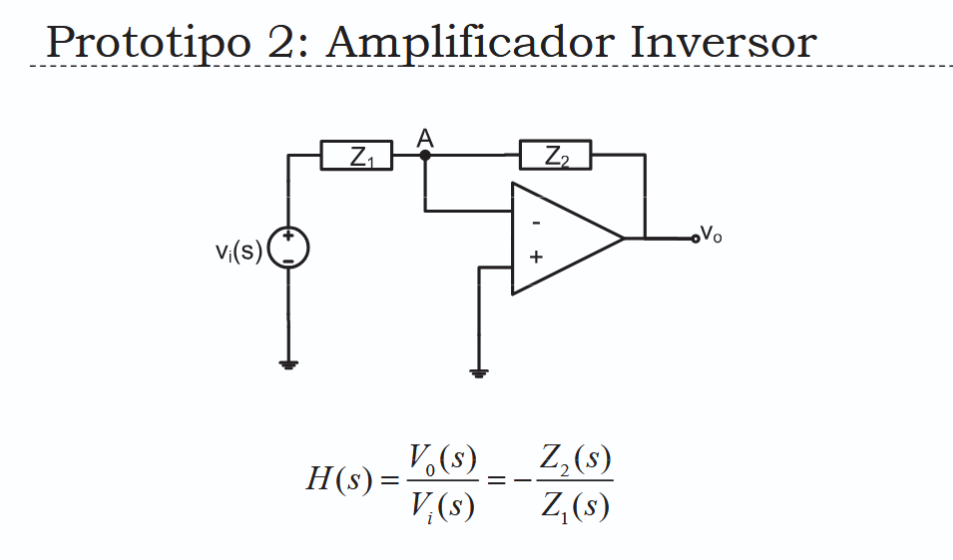
\includegraphics[width=0.5\textwidth]{Auxiliar_8_4}
\end{center}

Recordando la función de transferencia del enunciado tenemos que:
\[
T(s) = \frac{300(s+10)}{s(s+200)}
\]
Observamos que se puede factorizar como el producto de dos bloques en casacada.
\[
T(s) = \underbrace{\frac{300}{s}}_{H_1(s)} \cdot \underbrace{\frac{s+10}{s+200}}_{H_2(s)}
\]

Analizando la topología del OPAMP inversor, su función de transferencia general es:
\[
H(s) = -\frac{Z_2(s)}{Z_1(s)}
\]

Para implementar \( H_1(s) \), tomamos:
\[
H_1(s) = \frac{Z_2(s)}{Z_1(s)} = \frac{300}{s}
\implies Z_2(s) = \frac{300}{s}, \quad Z_1(s) = 1
\]
Donde observamos que correspode a un condensador de valor \( C_2 = \frac{1}{300} \,\text{F} \) (ya que la impedancia de un condensador es \( 1/(sC) \)), y una resistencia de \( 1\,\Omega \).

De manera análoga, para implementar \( H_2(s) \), consideramos:
\[
H_2(s) = \frac{Z_4(s)}{Z_3(s)} = \frac{s+10}{s+200}
= \frac{1 + \frac{10}{s}}{1 + \frac{200}{s}}
\]
Por lo tanto, basta tomar:
\[
Z_4(s) = 1 + \frac{10}{s} \qquad \text{y} \qquad Z_3(s) = 1 + \frac{200}{s}
\]
Esto corresponde a una condensador y una resistencia en serie. Finalmente, el circuito con dos OPAMPs inversores que implementa la función de transferencia \( T(s) \) es:

\begin{center}
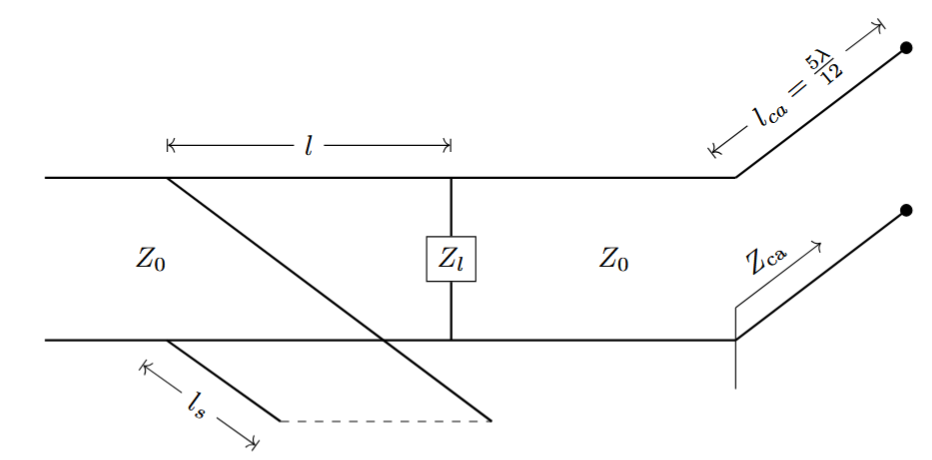
\includegraphics[width=0.6\textwidth]{Auxiliar_8_5}
\end{center}

Por lo tanto, el filtro diseñado con dos OPAMPs cumple con la función de transferencia requerida.
    \end{enumerate}
\end{solution}
%%%%%%%%%%%%%%%%%%%%%%%%%%%%%
\question Construir el diagrama de Bode de la función
\begin{equation}
    T(s) = 5000\,\frac{(s + 100)}{s^2 + 400s + 500^2}
\end{equation}

%%%%%%%%%%%%%%%%%%%%%%%%%%%%%%
\begin{solution}
   La función de transferencia es:
\begin{equation}
    T(s) = 5000\,\frac{(s+100)}{s^2 + 400s + 500^2}
\end{equation}

Para el análisis de Bode, recordemos que siempre trabajamos en régimen permanente, por lo que se evalúa en \( s = j\omega \):
\[
T(j\omega) = \frac{5000(j\omega + 100)}{(j\omega)^2 + 400j\omega + 500^2}
\]

Es conveniente expresar la función en términos de factores normalizados, para poder utilizar las tablas de Bode:
\begin{align*}
T(j\omega) &= \frac{5000(j\omega + 100)}{(j\omega)^2 + 400j\omega + 500^{2}} 
\end{align*}

La idea es factorizar con tal de formar terminos conocidos en las tablas de diagramas de fase y magnitud que adjunto a continuacion.

\begin{center}
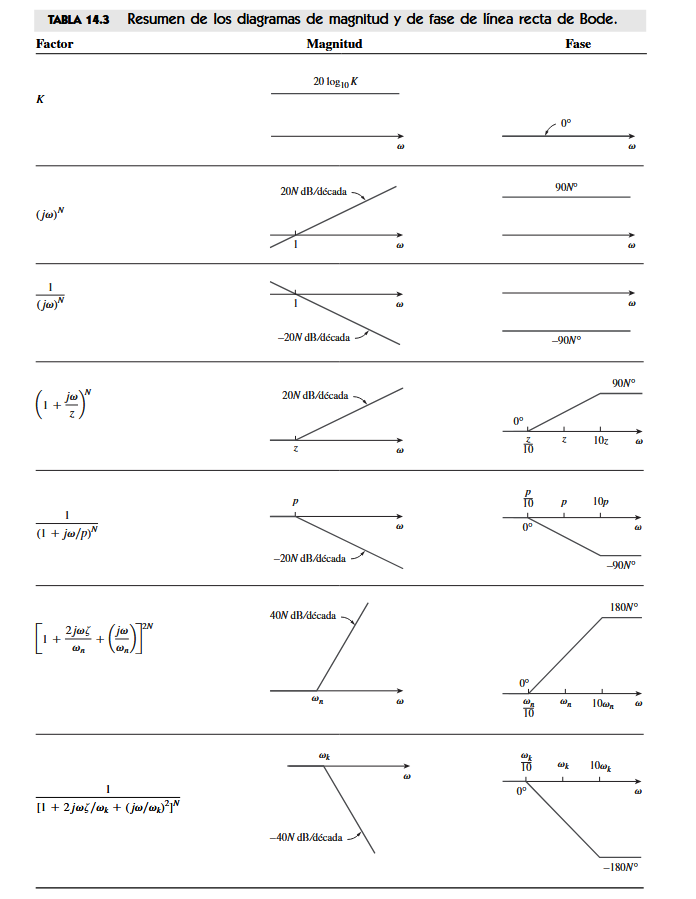
\includegraphics[width=0.7\textwidth]{Auxiliar_8_6}
\end{center}
Con lo que podemos identificar los términos relevantes para el trazado de Bode. Primero, identificamos el numerador y denominador y reescribimos de la siguiente manera:
\begin{align*}
T(j\omega) &= \frac{5000(j\omega + 100)}{(j\omega)^2 + 400j\omega + 500^{2}} \\
&=  \frac{5000 \cdot 100 \cdot \left(1+ \frac{j\omega}{100}\right)}{(j\omega)^2 + 400j\omega + 500^{2}}
\end{align*}
De la misma manera se divide por \(500^2\) para normalizar, tal que:

\begin{align}
    T(j\omega) &= \frac{5000 \cdot 100 \left(1+ \frac{j\omega}{100}\right)}{(j\omega)^2 + 400j\omega + 500^{2}} \\
    &= \frac{5000 \cdot 100}{500^{2}} \frac{1 + \frac{j\omega}{100}}{\left( \frac{j\omega}{500} \right)^2 + 400 \frac{j\omega}{500^{2}} + 1}\\
    &= 2 \cdot \frac{1 + \frac{j\omega}{100}}{\left( \frac{j\omega}{500} \right)^2 + 400 \frac{j\omega}{500^{2}} + 1 }
\end{align}
Luego aplicamos el logaritmo para obtener el módulo en decibeles a lo anterior, tal que:

\begin{align*}
    20 \log_{10} |T(j\omega)| &= 20 \log_{10} (2) + 20 \log_{10} \left| 1 + \frac{j\omega}{100} \right| - 20 \log_{10} \left| \left( 1 + \frac{j\omega}{500} \right)^2 + \frac{400}{500^2} j\omega + 1 \right|
\end{align*}
\begin{center}
    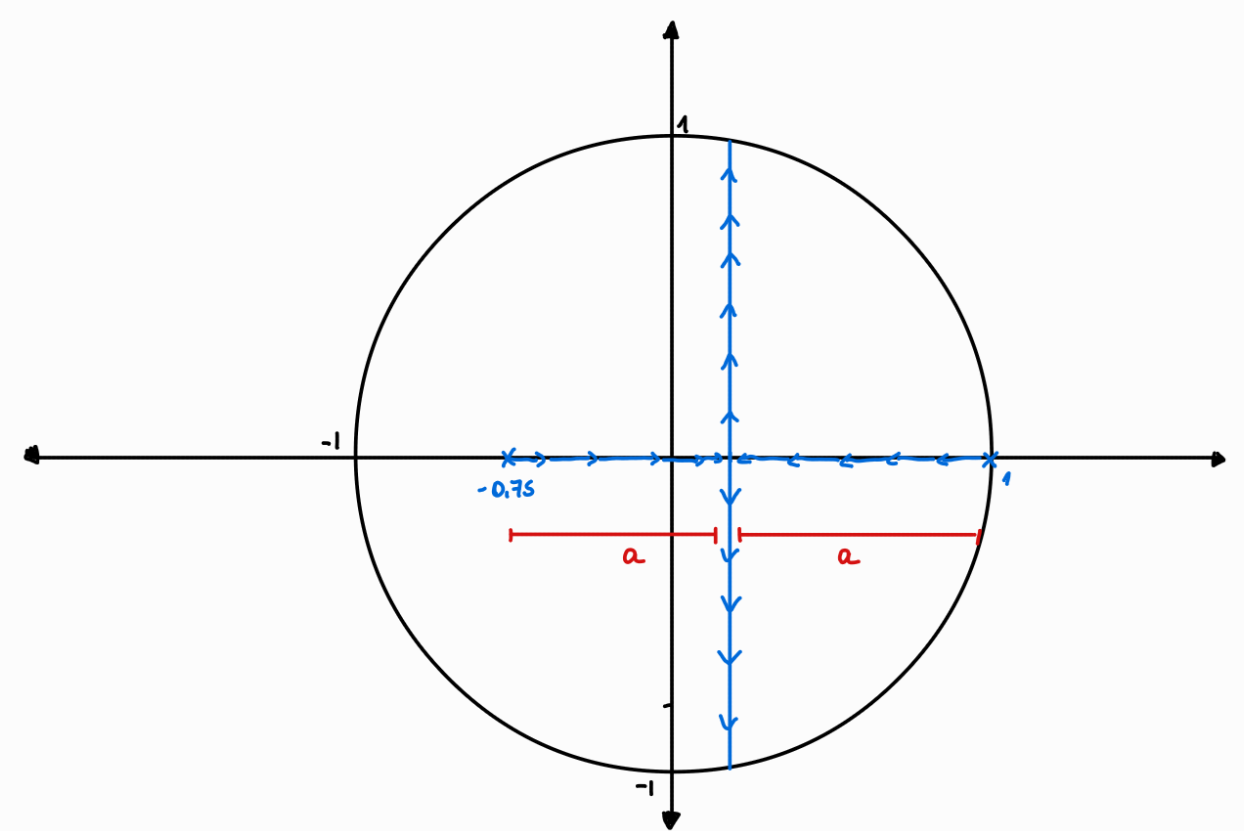
\includegraphics[width=0.6\textwidth]{Auxiliar_8_7}
\end{center}
Luego es posible graficar al superponer cada grafico anterior es importante tener en cuenta la caida de decibeles de cada bloque, dado que el denominador($40 [db/decada]$). tiene una mayor pendiente que el numerador ($20 [db/decada]$). Por otro lado para la fase se emplea la misma lógica, por lo que se tiene lo siguiente
\begin{center}
    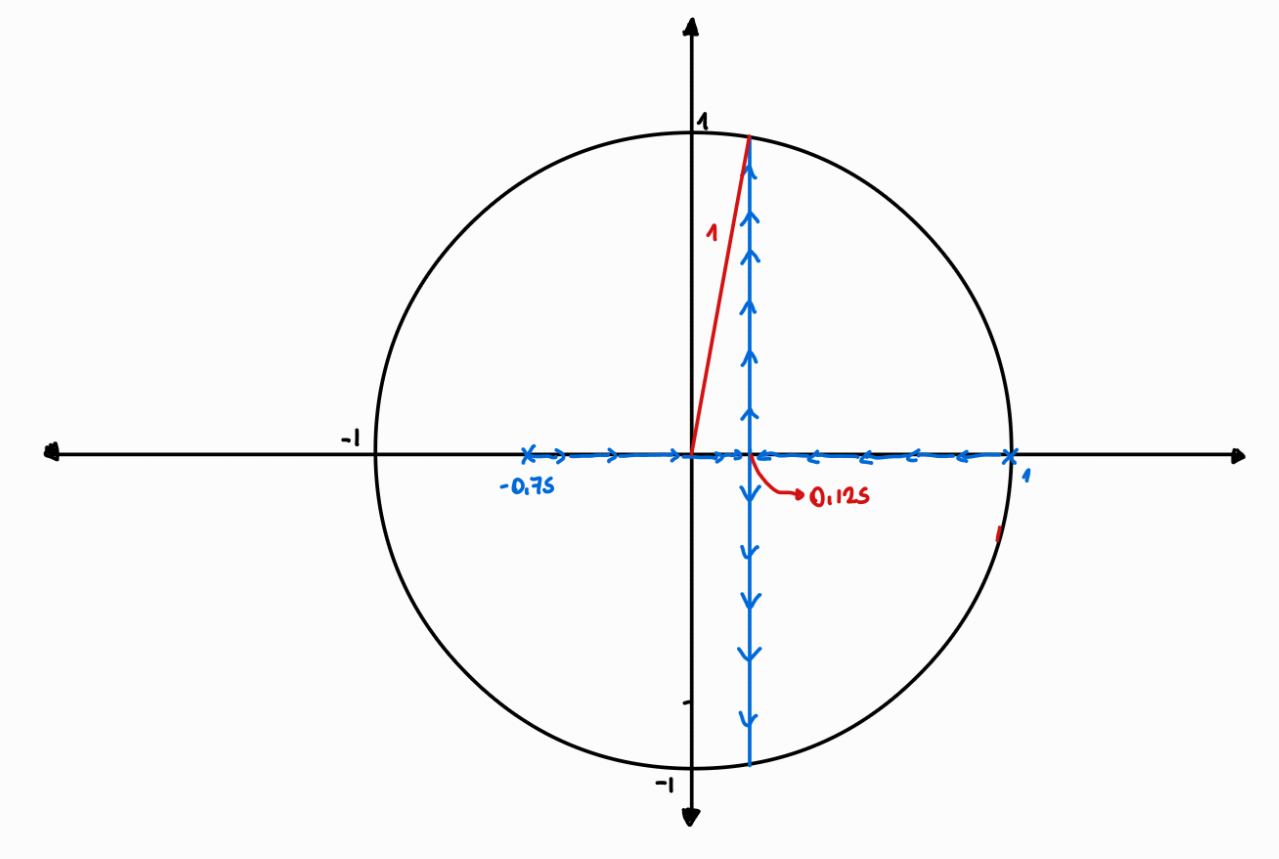
\includegraphics[width=0.6\textwidth]{Auxiliar_8_8}
\end{center}
\end{solution}
%%%%%%%%%%%%%%%%%%%%%%%%%%%%%%:
\question Dibuje el diagrama de Bode de magnitud y fase para la siguiente función de transferencia:
\begin{equation}
    T(s) = \frac{5s}{2(s+1)(s+5)^2(s+10)}
\end{equation}
%%%%%%%%%%%%%%%%%%%%%%%%%%%%%%%
\begin{solution}
 La función de transferencia es:
\begin{equation}
    T(s) = \frac{5s}{2(s+1)(s+5)^2(s+10)}
\end{equation}

Siguiendo el mismo procedimiento que en el ejemplo anterior, se tiene que para \( s = j\omega \):

\[
T(j\omega) = \frac{5j\omega}{2(j\omega+1)(j\omega+5)^2(j\omega+10)}
\]

Esto se puede expresar como una multiplicación de factores elementales:
\[
T(j\omega) = \frac{5}{2} \cdot (j\omega) \cdot \frac{1}{j\omega+1} \cdot \frac{1}{(j\omega+5)^2} \cdot \frac{1}{j\omega+10}
\]

Normalizando cada factor, tenemos:
\[
T(j\omega) = \frac{5}{2} \cdot (j\omega) \cdot \frac{1}{j\omega+1} \cdot \frac{1}{5^2 \left( \frac{j\omega}{5} + 1 \right)^2} \cdot \frac{1}{10 \left( \frac{j\omega}{10} + 1 \right)}
\]

Reuniendo constantes:
\[
T(j\omega) = \frac{5}{2 \cdot 25 \cdot 10} \cdot (j\omega) \cdot \frac{1}{j\omega+1} \cdot \frac{1}{\left( \frac{j\omega}{5} + 1 \right)^2} \cdot \frac{1}{\left( \frac{j\omega}{10} + 1 \right)}
\]
\[
= \frac{5}{500} \cdot (j\omega) \cdot \frac{1}{j\omega+1} \cdot \frac{1}{\left( \frac{j\omega}{5} + 1 \right)^2} \cdot \frac{1}{\left( \frac{j\omega}{10} + 1 \right)}
\]
\[
= 0.01 \cdot (j\omega) \cdot \frac{1}{j\omega+1} \cdot \frac{1}{\left( \frac{j\omega}{5} + 1 \right)^2} \cdot \frac{1}{\left( \frac{j\omega}{10} + 1 \right)}
\]

Por lo tanto, el módulo en decibeles es:
\[
20\log_{10} \left| T(j\omega) \right| = 20\log_{10}(0.01) + 20\log_{10}|j\omega| - 20\log_{10}|j\omega + 1| - 40\log_{10} \left| \frac{j\omega}{5} + 1 \right| - 20\log_{10} \left| \frac{j\omega}{10} + 1 \right|
\]

Luego de manera grafica tenemos que:
\begin{center}
    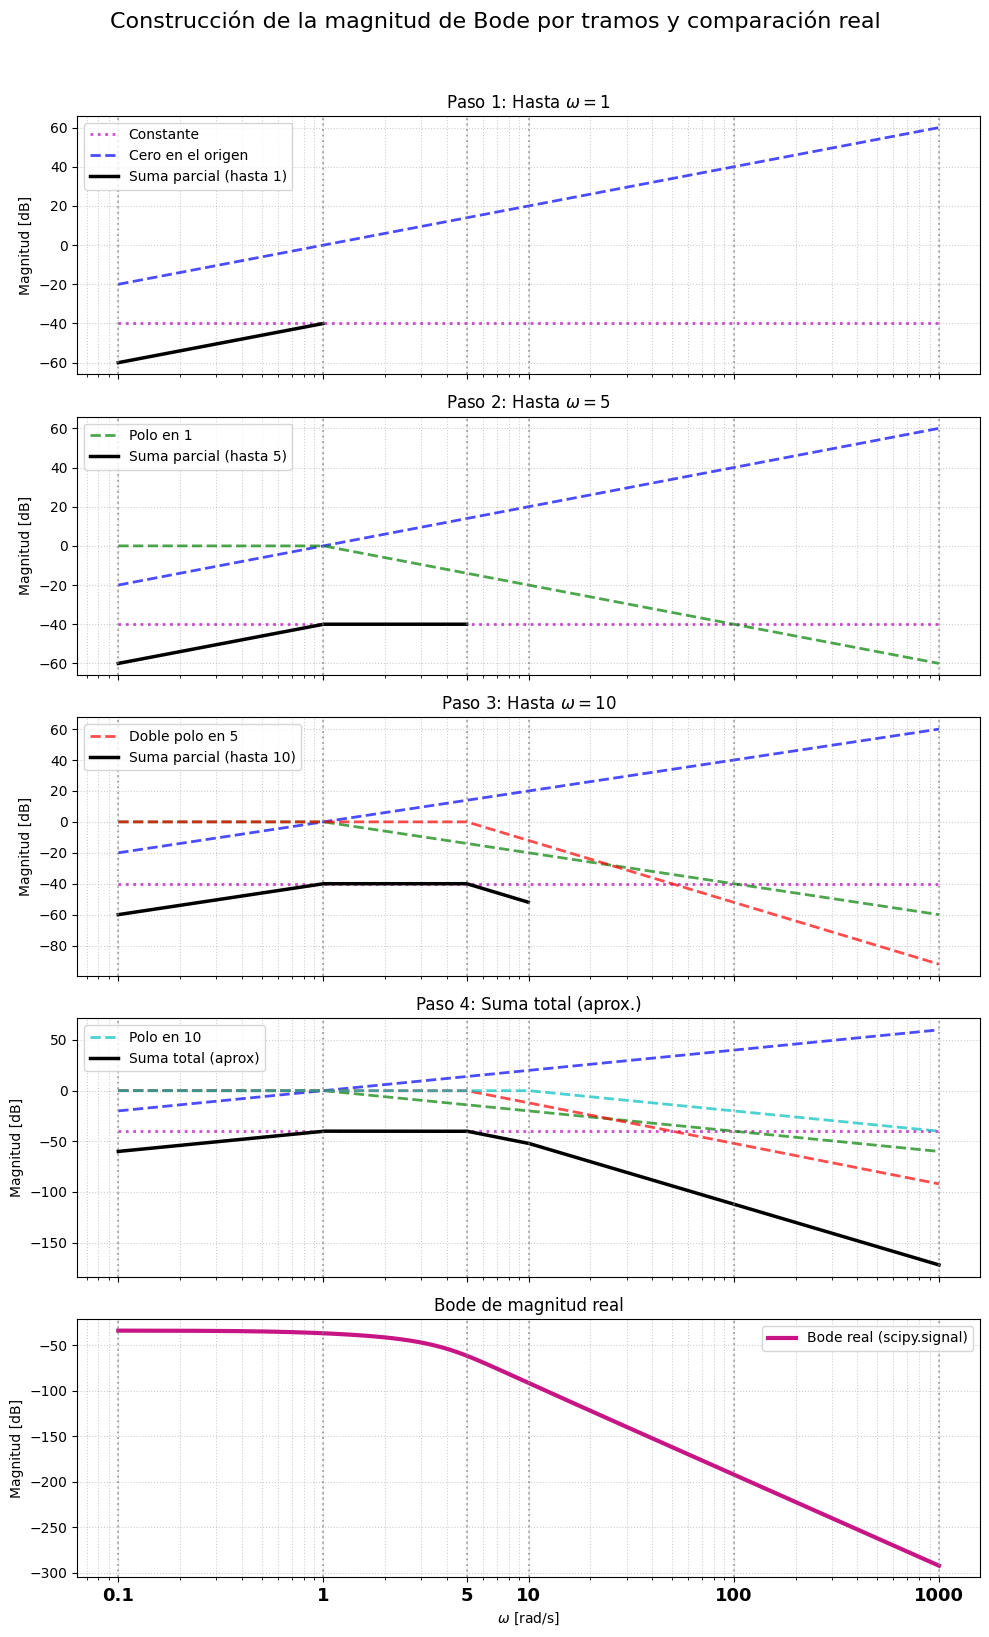
\includegraphics[width=0.6\textwidth]{Auxiliar_8_9}
\end{center}
Para la fase, se tiene:
\begin{center}
    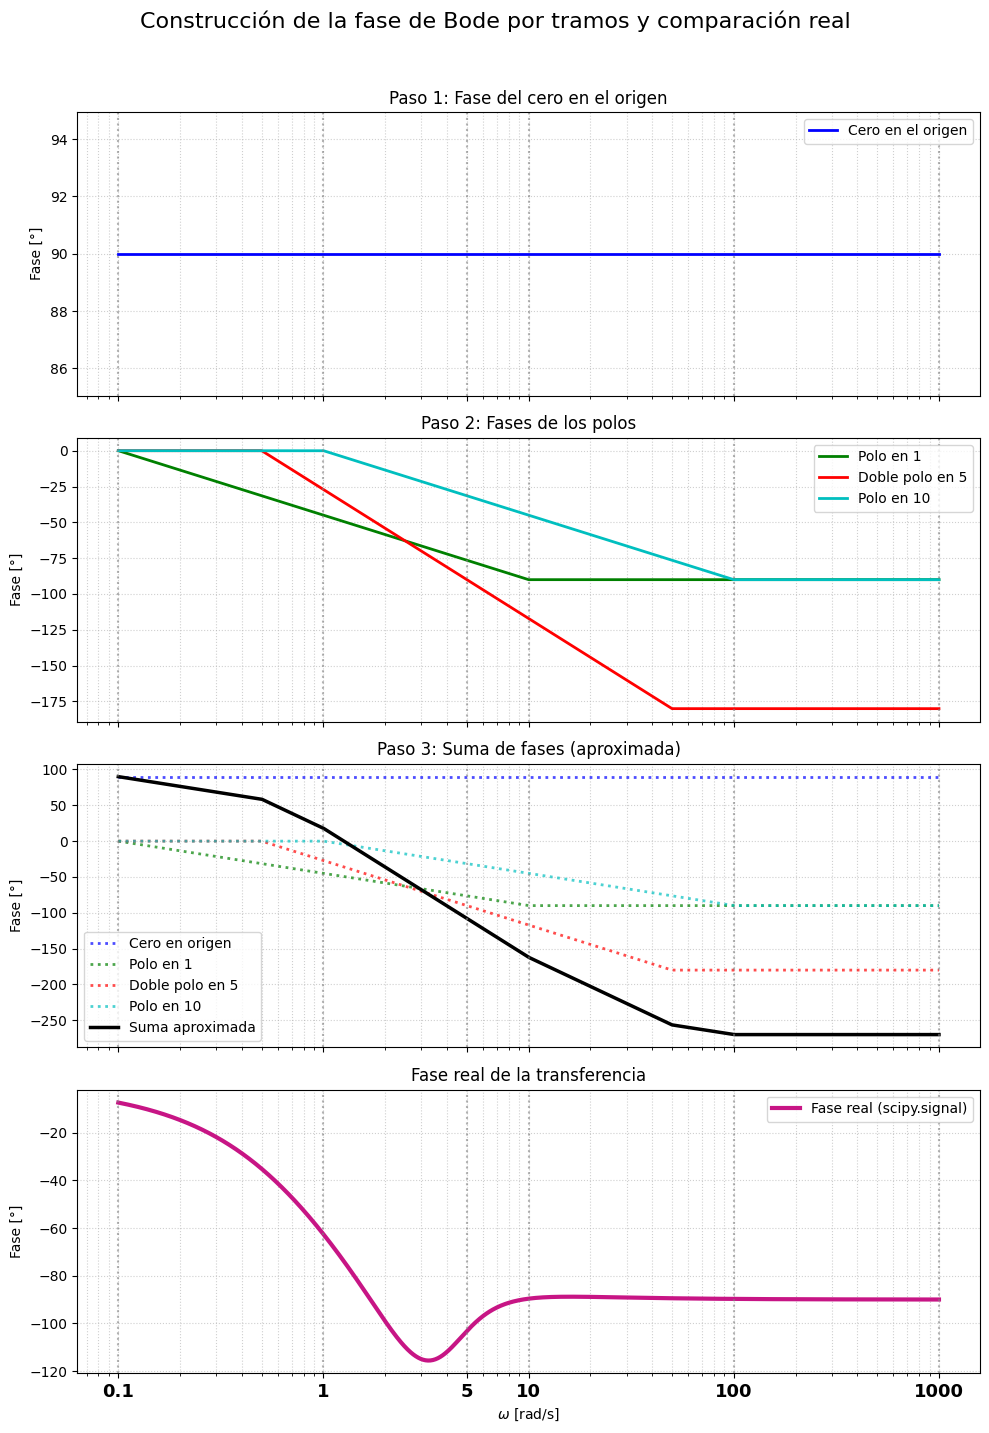
\includegraphics[width=0.6\textwidth]{Auxiliar_8_10}
\end{center}


\end{solution}
%%%%%%%%%%%%%%%%%%%%%%%%%%%%%%%

\question En el circuito de la Figura~\ref{fig:esquema-filtro}, los condensadores están descargados. Se pide:

\begin{figure}[h!]
    \centering
    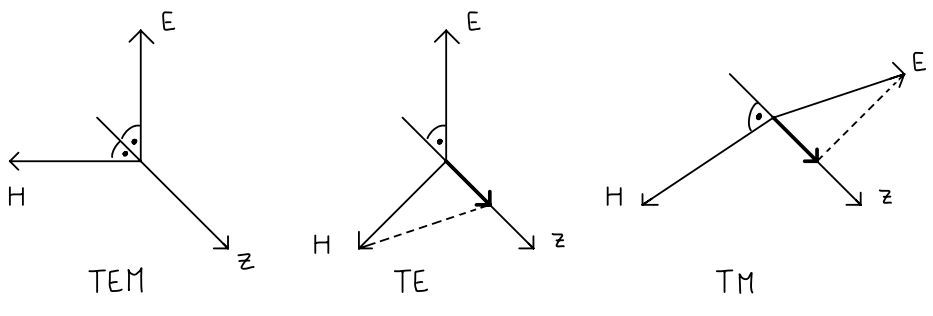
\includegraphics[width=0.55\textwidth]{Auxiliar_8_2}
    \caption{Esquema figura}
    \label{fig:esquema-filtro}
\end{figure}

\begin{enumerate}
    \item Encontrar la función de transferencia \( V_2(s)/V_1(s) \).
    \item Seleccionar valores de \( R \) y \( C \) tal que los polos de la función de transferencia sean aproximadamente \( s_1 = -2618~[\text{rad/s}] \) y \( s_2 = -382~[\text{rad/s}] \).
\end{enumerate}
%%%%%%%%%%%%%%%%%%%%%%%%%%%%%%%
\begin{solution}
    \begin{itemize}
        \item  Para resolver el circuito, aplicamos las Leyes de Kirchhoff en el dominio de Laplace, considerando los capacitores descargados inicialmente. Nombramos \( I_1(s) \) como la corriente por el primer e \( I_2(s) \) como la corriente de la otra malla. Luego para la primera malla tenemos que:
\begin{center}
    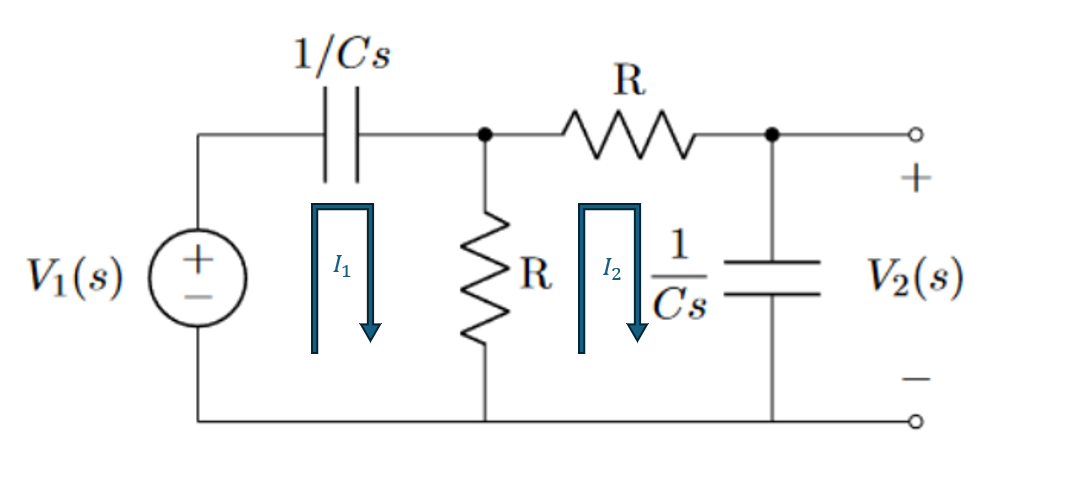
\includegraphics[width=0.6\textwidth]{Auxiliar_8_12}
\end{center}
\begin{align}
    -V_1(s) + I_1 \frac{1}{Cs} + R(I_1 - I_2) = 0
\end{align}

Para la malla 2 tenemos que despejando \( I_2 \) en función de \( I_1 \):
\begin{align}
  R(I_2 - I_1) + R I_2 + I_2 \frac{1}{Cs} = 0 \\
    I_2(R + \frac{1}{Cs}) = I_1 R \\
    I_2 = \frac{I_1 R}{R + \frac{1}{Cs}} = I_1 \left( \frac{RCs}{2RCs + 1} \right)
\end{align}
Luego sustituyendo \( I_2 \) en la ecuación de la malla 1, tenemos que:
\begin{align*}
    &-V_1(s) + I_1 \cdot \frac{1}{Cs} + R(I_1 - I_2) = 0 \\
    &I_1 + RCs \, I_1 - RCs \, I_2 = V_1(s) Cs \\
    &I_1 (1 + RCs) - RCs\, I_2 = V_1(s) Cs \\
    &I_1 (1 + RCs) - RCs \, I_1 \left( \frac{RCs}{2RCs + 1} \right) = V_1(s) Cs \\
    &I_1 \left[ 1 + RCs - \frac{(RCs)^2}{2RCs + 1} \right] = V_1(s) Cs \\
    &I_1 \left[ \frac{3RCs + (RCs)^2 + 1}{2RCs + 1} \right] = V_1(s) Cs \\
    &I_1 = \left[ \frac{V_1(s) \cdot Cs (2RCs + 1)}{3RCs + (RCs)^2 + 1} \right]
\end{align*}


Luego \( I_{2} \) sera lo siguiente:
\begin{align}
    I_2 &= \frac{I_1 R}{R + \frac{1}{Cs}} = I_1 \left( \frac{RCs}{2RCs + 1} \right)\\
    &= \frac{V_1(s) \cdot Cs (2RCs + 1)}{3RCs + (RCs)^2 + 1} \cdot \left( \frac{RCs}{2RCs + 1} \right)\\
    &= \frac{V_1(s) \cdot R (Cs)^2}{3RCs + (RCs)^2 + 1}
\end{align}
luego tendremos que el voltaje en el capacitor de salida \( V_2(s) \) es:
\begin{align}
    V_2(s) &= \frac{1}{Cs} I_2(s) = \frac{1}{Cs} \cdot \frac{V_1(s) \cdot R (Cs)^2}{3RCs + (RCs)^2 + 1}\\
    &= \frac{V_1(s) \cdot R Cs}{3RCs + (RCs)^2 + 1}
\end{align}
Como buscamos la funcion de transferencia \( H(s) = \frac{V_2(s)}{V_1(s)} \), tenemos que reemplazando:
\begin{align}
    H(s) &= \frac{V_2(s)}{V_1(s)} = \frac{R Cs}{3RCs + (RCs)^2 + 1}
\end{align}
Luego se escribe de manera conveniente para dividiendo tanto numerador como denominador por \( (RC)^{2} \), dando como resultado que:
\begin{align}
    H(s) &= \frac{R Cs}{3RCs + (RCs)^2 + 1} = \frac{s}{\frac{3}{RC}s + s^2 + \frac{1}{(RC)^2}}\\
    &= \frac{s}{s^2 + \frac{3}{RC}s + \frac{1}{(RC)^2}}
\end{align}

Ahora se busca que los polos de la función de transferencia sean aproximadamente \( s_1 = -2618\,\mathrm{rad/s} \) y \( s_2 = -382\,\mathrm{rad/s} \). Es decir, que el denominador que buscamos sea:
\begin{align}
  H(s)= \frac{s}{s^2 + \frac{3}{RC}s + \frac{1}{(RC)^2}}= \frac{\frac{s}{RC}}{(s + 2618)(s + 382)}
\end{align}
Por lo que desarrollando el denominador de lo que se busca imponer tenemos que:
\begin{align}
    (s + 2618)(s + 382) &= s^2 + (2618 + 382)s + 2618 \cdot 382 \\
    &= s^2 + 2936s + 832.524
\end{align}
De esta manera el sistemas de ecuaciones que se debe resolver es:
\begin{align}
    \frac{3}{RC} &= 2936 \\
    \frac{1}{(RC)^2} &= 832.524
\end{align}

Así, existe un grado de libertad: al elegir un valor para \( R \), calculamos \( C \), o viceversa.

Por ejemplo, si elegimos \( R = 200\,\Omega \) se tendra que:
\begin{align}
    \frac{3}{200C} &= 2936 \\
    C &= \frac{3}{200 \cdot 2936} = 5.1 \cdot 10^{-5}\,\mathrm{F} = 51\,\mu\mathrm{F}
\end{align}

En conclusión, existen infinitas combinaciones de \( R \) y \( C \) que cumplen las condiciones para la ubicación de los polos; basta con que los productos \( RC \) y \( R \) respeten las ecuaciones anteriores.
\end{itemize}
\end{solution}

%%%%%%%%%%%%%%%%%%%%%%%%%%%%%%%%
\question Encuentre la función de transferencia \( H(s) = \frac{V_0}{V_s} \) asumiendo que los condensadores se encuentran descargados (ver Figura~\ref{fig:opamp-filtro}).

\begin{figure}[h!]
    \centering
    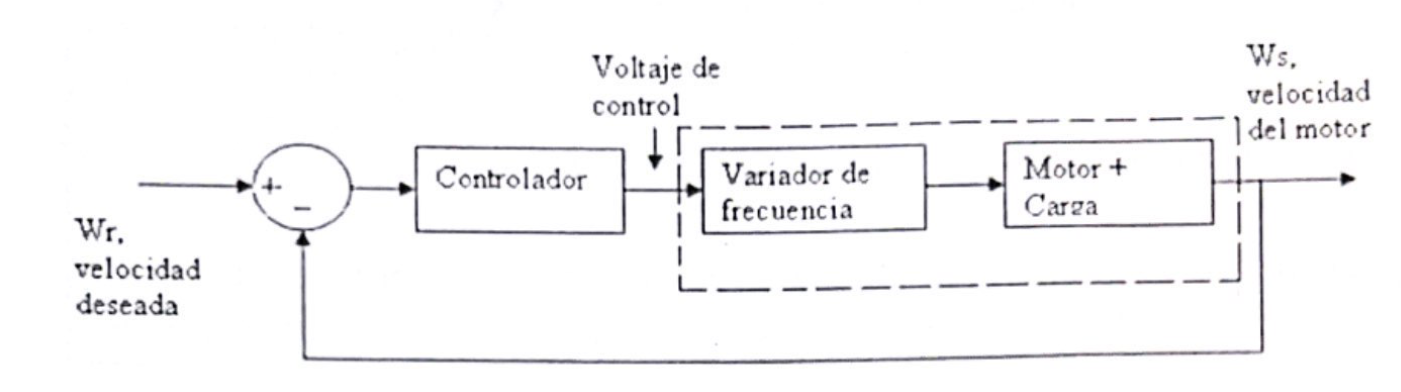
\includegraphics[width=0.6\textwidth]{Auxiliar_8_3}
    \caption{Circuito con amplificador operacional y condensadores descargados.}
    \label{fig:opamp-filtro}
\end{figure}

%%%%%%%%%%%%%%%%%%%%%%%%%%%%%%%%
\begin{solution}
    Para encontrar la función de transferencia \( H(s) = \frac{V_0(s)}{V_s(s)} \) del circuito con amplificador operacional y dos condensadores en serie en la rama de realimentación, se puede simplificar el análisis combinando los condensadores \( C_1 \) y \( C_2 \) en una sola capacitancia equivalente \( C_{eq} \).Primero, se reduce la rama de realimentación:
\begin{equation}
    C_{eq} = \left( \frac{1}{C_1} + \frac{1}{C_2} \right)^{-1} = \frac{C_1 C_2}{C_1 + C_2}
\end{equation}
Luego se definen diferentes nodos de interes, por lo tanto tenemos que:
\begin{center}
    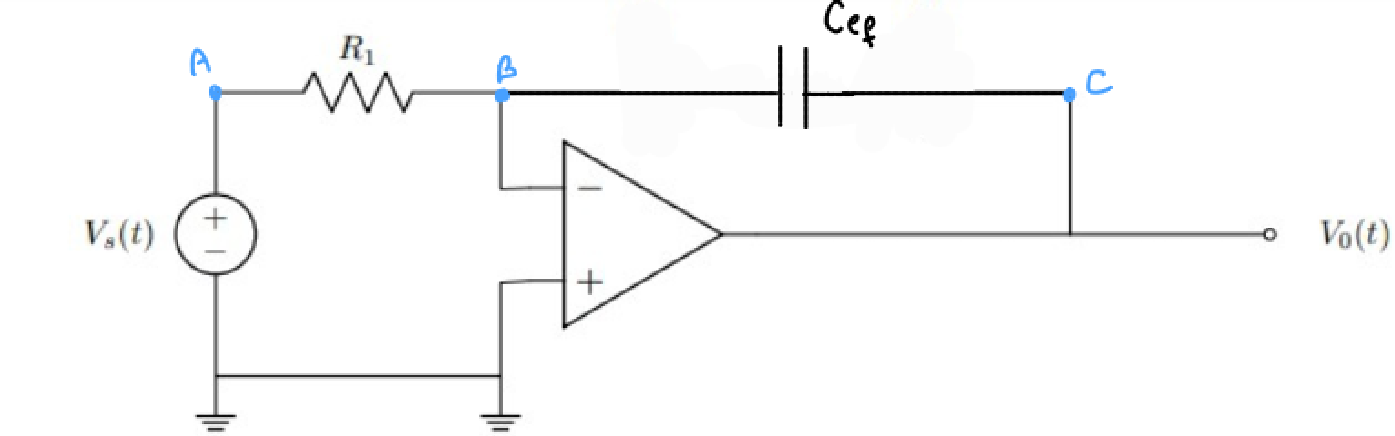
\includegraphics[width=0.6\textwidth]{Auxiliar_8_11}
\end{center}
De esta manera en el nodo B tenemos que  $i_1 = i_2$:
\begin{equation}
    \frac{V_a - V_b}{R_1} = \frac{V_b-V_c}{\frac{1}{C_{eq}}s}
\end{equation}
Pero sabemos que \( V_b = 0 \) (masa virtual), por lo que:
\begin{equation}
    \frac{V_a}{R_1} = -\frac{V_c}{\frac{1}{C_{eq}}s}
\end{equation}
Ademas tenemos que \( V_a = V_s \) y \( V_c = V_0 \) por lo que reemplazando tenemos que:
\begin{align}
    \frac{V_s}{R_1} &= -\frac{V_0}{\frac{1}{C_{eq}}s}\\
    &= -C_{eq}s V_0
\end{align}
Luego como queremos la funcion de transferencia tenemos que:
\begin{align}
    H(s) = \frac{V_0(s)}{V_s(s)} = \frac{-1}{R_{1} C_{eq} s}= -\frac{1}{R_1 s} \cdot \frac{C_2 + C_1}{C_1 C_2}
\end{align}
Obteniendo lo buscado. :

\end{solution}
%%%%%%%%%%%%%%%%%%%%%%%%%%%%%%%%
\end{questions}

\end{document}